\documentclass[10pt,letterpaper]{article}
% Copyright (c) 2026 Jonathan Yantis. Paper and original figures: CC BY 4.0.
\usepackage[margin=0.78in]{geometry}
\usepackage[T1]{fontenc}
\usepackage{lmodern,microtype,amsmath,amssymb,booktabs,array,graphicx}
\usepackage[colorlinks=true,linkcolor=blue,urlcolor=blue,citecolor=blue]{hyperref}
\usepackage{enumitem}
\setlist{nosep,leftmargin=*}
\setlength{\parskip}{0.3em}
\setlength{\parindent}{0pt}
\newcommand{\code}[1]{\texttt{\small #1}}
\newcommand{\us}{\ensuremath{\mu\mathrm{s}}}
\newcommand{\ns}{\ensuremath{\mathrm{ns}}}
\title{\vspace{-1.5em}A Raspberry Pi Time Server at the Edge of a BLE Timing Mesh\\
\large Measured M-HAT PPS Transfer and Prospects for USB and Reverse PTP Gateways}
\author{Jonathan Yantis}
\date{2 November 2026\\\small Author-review draft --- not publication-approved}
\begin{document}
\maketitle
\vspace{-1em}
\begin{abstract}
A Raspberry Pi can make a wireless timing mesh useful to existing NTP and PTP
clients without requiring those clients to implement Bluetooth timing.
We implement the path on a Pi 5 Model B and an nRF52840 Particle B504e M-HAT that receives
authenticated PToB timing and generates hardware-timer PPS through the HAT bus.
Linux GPIO PPS feeds chrony, with network NTP supplying coarse UTC seconds;
guarded system-to-PHC transfer prepares an Ethernet PTP server.
After a 120-second settled period, one fixed 600.026-second window retained
600 of 600 new PPS assertions with one source cohort and no observed gaps or
service restarts. GPIO assertion phase against the disciplined Pi clock had
872 ns RMS, 4.809 \us{} absolute P99 and 7.017 \us{} maximum; all tails remain.
Chrony's separately sampled RMS estimate had a 72 ns median. These are different
feedback-path metrics, not independently measured UTC or output accuracy.
A causal USB/SOF bridge modeled on the existing macOS client and an external
PTP-to-PToB source are evaluated as future designs. Neither Pi USB precision nor
the reverse path has been measured. The intended result is a reproducible integration
study and an error-aware roadmap, rather than a sub-microsecond accuracy claim.
\end{abstract}

\section{What a Pi time-server user can build}
PToB distributes a source-scoped clock across compatible BLE receivers. For a
Pi time-server user, the practical attraction is a wireless reference link while
retaining familiar Linux tools and network clients. The engineering problem is
not simply to receive a time value: it is to associate that value with a
physical event, carry its original validity interval to the host, and withdraw
the network claim when its authority or timing path disappears.

The tested target is an ordinary Raspberry Pi 5 Model B, rather than a CM4 or
a specially wired Ethernet timing carrier. A Particle M-HAT contains the B504e
variant of the nRF52840. Its custom Zephyr receiver reuses the repository's
G1/RC7 precision reception and authenticated admission, then generates PPS
without relying on Linux to schedule the edge. The HAT firmware is currently
an RC receiver. It is not a PToB GM implementation.

This study addresses three questions. First, does the complete BLE-to-HAT-to-Pi
clock path operate continuously for a prescribed ten minutes, and what do its
observed RMS and tails mean? Second, could a USB event bridge avoid the present
GPIO interrupt capture path? Third, could an externally synchronized PTP gateway
instead become a source for the BLE mesh? The last two are design analyses;
their performance cannot be inferred by reversing the measured arrows.

\begin{figure}[ht]
\centering\small
\begin{tabular}{c@{ $\longrightarrow$ }c@{ $\longrightarrow$ }c@{ $\longrightarrow$ }c}
\fbox{BLE GM / mesh} & \fbox{M-HAT map + PPS} & \fbox{GPIO + chrony} & \fbox{NTP / PHC--PTP}\\[0.7em]
\multicolumn{4}{c}{Implemented forward path; Ethernet endpoint accuracy not yet measured}\\[0.8em]
\fbox{External PTP} & \fbox{Receiver PHC} & \fbox{Timer bridge + GM} & \fbox{PToB mesh}\\[0.7em]
\multicolumn{4}{c}{Proposed reverse path; bridge and M-HAT GM mode require implementation}
\end{tabular}
\caption{The two directions have different clock owners and measured boundaries.
Changing an arrow's direction requires a new source association and validity contract.}
\label{fig:directions}
\end{figure}

\section{The implemented clock chain}
\subsection{Radio reception and hardware PPS}
The M-HAT uses nRF52840 RADIO event capture through PPI into a dedicated
16 MHz TIMER3. Authenticated original/follow-up associations enter the shared
receiver discipline and produce an immutable source map. TIMER compare,
PPI and GPIOTE generate a 10 ms pulse as a hardware one-shot. Foreground work
plans the event but does not toggle the pin at the desired second. Nordic
documents the timer, event interconnect and USB peripheral mechanisms
\cite{nordic}; counter resolution alone does not calibrate radio or board delay.

The planner continually reprojects the latest admitted map until the edge is
within 20 ms, checks a minimum lead, and chooses the nearest attainable timer
tick. Both rise and fall must remain within the original map, source and session
permissions. Original source and session expiry remain authoritative for every generated
pulse; the planner cannot extend permission to complete a pulse.


The timer's 62.5 ns step gives an ideal nearest-edge error of at most half a
tick. A uniform, independent quantization model would have
\[
 \sigma_q=\frac{62.5}{\sqrt{12}}\ \ns \simeq18.0\ \ns .
\]
Fractional source phase can average below one tick in a suitable estimator.
Neither independence nor absence of bias follows from timer resolution.
Averaging cannot remove fixed RF, GPIO, PHY or cable delay.

\subsection{Wiring and Linux ownership}
\begin{table}[ht]
\centering\small
\caption{Implemented M-HAT bus paths. GPIO4 is power control, not PPS.}
\begin{tabular}{llll}
\toprule Function & nRF52840 & HAT/module signal & Pi header\\
\midrule
PPS rise/fall & P1.02 & D2 / RTS & GPIO16, pin 36\\
Diagnostic TX & P0.06 & D9 / TXD & GPIO15 RX, pin 10\\
Diagnostic RX & P0.08 & D10 / RXD & GPIO14 TX, pin 8\\
Bus enable & P0.03 & A0 / SEL & internal switch\\
\bottomrule
\end{tabular}
\end{table}
The GPIO stack carries PPS and UART diagnostics; it does not carry USB.
UART is 115200 baud, 8N1 with no flow control, because RTS is used for PPS.
BLE requires the separate BT antenna. No GPIO jumper is needed for this route.
Existing power arrangements must remain valid when attaching a USB data cable.

Linux \code{pps-gpio} supplies kernel assertion timestamps
\cite{linuxpps,ppsgpio}. Chrony owns \code{CLOCK\_REALTIME}; PPS supplies phase,
and NTP supplies coarse second numbering. A private UART collector validates
the exact device and installed source, records source/root/boot/epoch/parent,
and reports whether current admission, PPS and chrony selection form a complete
path. Reporting is not an additional clock writer.

The prepared configuration uses
\begin{quote}\small\ttfamily
refclock PPS /dev/pps-ptob refid PTOB poll 0 dpoll 0 prefer
\end{quote}
alongside the configured NTP pool. Debian's \code{tzdata-legacy} supplies the
\code{right/UTC} leap database on this image \cite{debiantz}; the kernel's operating
TAI--UTC offset must be valid before the Ethernet server is admitted.
A one-second source poll does not provide
multi-sample refclock averaging by itself: chrony limits that filter to available
driver polls. Its tracking RMS, regression residual and assumed measurement
precision are different quantities \cite{chrony}. The prepared Pi runs its
performance governor, assigns the PPS GPIO IRQ to CPU3, and confines the
observer and gateway services to CPUs0--2. These are reported conditions, not
proof that unrelated work cannot delay an interrupt.

\subsection{NTP and PTP serving}
A single owned chrony instance can serve NTP from the disciplined system clock.
The Ethernet design transfers system time into the native PHC before permitting
a server-only PTP process. It explicitly handles the operating TAI--UTC offset,
source generation, stale supervisors and child cleanup. It never creates a
second system-clock servo. LinuxPTP documents the distinct PHC and system clock
directions and startup-step behavior \cite{phc2sys}.

On this Pi, \code{gem-ptp-timer} reports no external timestamp inputs, periodic
outputs or configurable timing pins. Ethernet packet timestamp support therefore
does not create a hardware PPS capture path. The current system-to-PHC
midpoint check is a coarse readiness fence; its 50 \us{} threshold is not a
sub-microsecond qualification. An unconnected Ethernet port cannot establish
end-to-end Ethernet performance.

The separate Wi-Fi PTP service uses software timestamps and an ARB timescale,
without permission to discipline the system. Valid NTP replies or matched PTP
Sync/Follow\_Up messages establish protocol health. They do not measure the
remote endpoint's UTC error or make the wireless packet path equivalent to
Ethernet hardware timestamping. Clock class, variance and traceability must
remain conservative until independently established.

\subsection{A deployment sequence for existing Pi servers}
A Pi user should first verify an exact compatible HAT, retain bootloader recovery,
and check the PPS pin assignment against the carrier rather than assuming all
Pi timing designs expose the same pins. Provision enrollment independently from
runtime mesh selection: the production image discovers a local context and
requires fresh authenticated admission when that context changes. A hard-coded
mesh identifier is not a durable source-selection strategy.

Next establish the source-to-PPS path before enabling network claims. Check that
root, root boot and source epoch are current, the receiver map is admitted,
assertion sequence advances at the expected rate, and chrony actually selects
PTOB with normal leap status. Keep NTP for second numbering and record the
coarse UTC relationship; a PPS-only lock cannot resolve an unknown whole second.
Service process state alone cannot replace these checks.

Finally qualify output separately. A native PHC capability inventory determines
whether hardware external PPS capture is possible. An Ethernet peer and a
measurement reference are needed before a system-to-PHC health residual becomes
an output-performance result. A startup or source-change test must observe
withdrawal, re-admission and recovery, not only a low steady-state RMS. This
sequence also allows existing GNSS/NTP/PTP users to keep their established
reference as a shadow witness while evaluating a mesh input.

\section{Measurement contract and experimental populations}
For assertion timestamp \(T_i\), define the signed phase
\[
 r_i=T_i-\operatorname{round}(T_i/\mathrm{s})\,\mathrm{s}.
\]
This is a software timestamp relative to the system clock being disciplined.
It includes the physical pulse's arrival and capture delay, radio/map and
timer errors, and the current system-clock correction. It is not an external
measurement of either absolute PPS or UTC.

We retain the mean, RMS and population standard deviation:
\[
 \bar r=N^{-1}\sum_i r_i,\qquad
 R=\sqrt{N^{-1}\sum_i r_i^2},\qquad
 \sigma=\sqrt{N^{-1}\sum_i(r_i-\bar r)^2}.
\]
RMS retains bias. Absolute P99 uses nearest rank
\(\lceil0.99N\rceil\); strict exceedance counts use \(>1\), \(>2\) and
\(>5\) \us. With 600 pulses, one P99 point cannot characterize a rare-event
distribution or guarantee a maximum beyond the observed window.

The observer polls cached sysfs assertions at 20 Hz and retains integer
nanoseconds and kernel sequences. One initially cached assertion is a seed,
not a newly captured pulse. Sequence skips distinguish events unseen by the
observer from nominal pulse slots without an assertion. One-Hz source and
quality snapshots describe lineage, fit age, chrony and transfer state.
Repeated tracking estimates are not independent updates. A conditional
source-eligible subset requires bracketing fresh, same-cohort observations;
it cannot certify exact-event authentication.

The experiment required a settled admitted cohort before a fixed
600-second measurement. Its root, root boot, source epoch, selected parent and
HAT boot must remain current, with fresh PPS and unchanged configuration and
clock ownership. A source change ends the qualification attempt; any subsequent
attempt begins after fresh admission and settling. Selection is by continuity
and a prescribed duration, never by error magnitude. The selected evidence
contains the entire final window. Availability eligibility places no threshold
on phase magnitude, so a continuous run may still exceed the precision objective.

\section{Final fixed-window observations}
\subsection{Conditions and continuity}
The Pi ran kernel \code{6.18.50+rpt-rpi-2712}, M-HAT firmware 0.5.5, the
one-second chrony PPS configuration above, performance governor and RP1 PCIe
L1 enabled. The observer used CPUs0--2; the PPS GPIO IRQ used CPU3. Normal UART
diagnostics, history collection, system-to-PHC transfer and PTP services remained
active. No trace probe, firmware update, clock-setting change or service restart
was introduced during acquisition. Source/image and configuration hashes are
recorded in the selected manifest; hashes establish identity rather than precision.

A continuous 120.041-second warmup preceded the fixed 600.026-second window.
We retained 600 new assertions for 600 nominal pulse opportunities, one excluded
cached seed, 599 new-to-new periods and 600 quality snapshots. All snapshots
showed fresh admitted timing, selected PTOB with normal leap state, fresh running
PHC transfer and a fresh ready/running Ethernet PTP guard. The full source cohort
remained unchanged. There were no observed sequence skips, missing nominal slots,
source transitions or in-window guard-generation changes. Boundary configuration
hashes and effective chrony settings matched; service identities and restart counts
matched across 41 observations. Acquisition and export error counts were zero.
This is finite-window continuity, not an endurance result.

\begin{table}[ht]
\centering\small
\caption{Complete final populations. Values describe the Pi feedback path;
they do not measure independent electrical or UTC error.}
\begin{tabular}{lrrrr}
\toprule Population & $N$ & Bias (ns) & RMS (ns) & $|\cdot|$ P99 / max (ns)\\
\midrule
GPIO assertion phase & 600 & $+2.063$ & 872.002 & 4809 / 7017\\
Consecutive period minus 1 s & 599 & $+1.905$ & 1106.541 & 6606 / 7777\\
Chrony last offset, distinct updates & 597 & $-9.325$ & 423.387 & 2521 / 3562\\
\bottomrule
\end{tabular}
\label{tab:phase}
\end{table}

\subsection{RMS, tails and internal estimates}
The GPIO phase population standard deviation was 871.999 ns, close to its
872.002 ns RMS because its mean was only $+2.063$ ns. Strict absolute exceedance
counts above 1, 2 and 5 \us{} were 46, 19 and 5 of 600, respectively. Thus 554/600
observations were within 1 \us{}, while absolute P99 was 4.809 \us{} and the
maximum was 7.017 \us. Every point contributes to the table and figure.
The five observations above 5 \us{} occurred within a 63-second portion of
the window. Continuous source admission did not eliminate timing tails.

\begin{figure}[ht]
\centering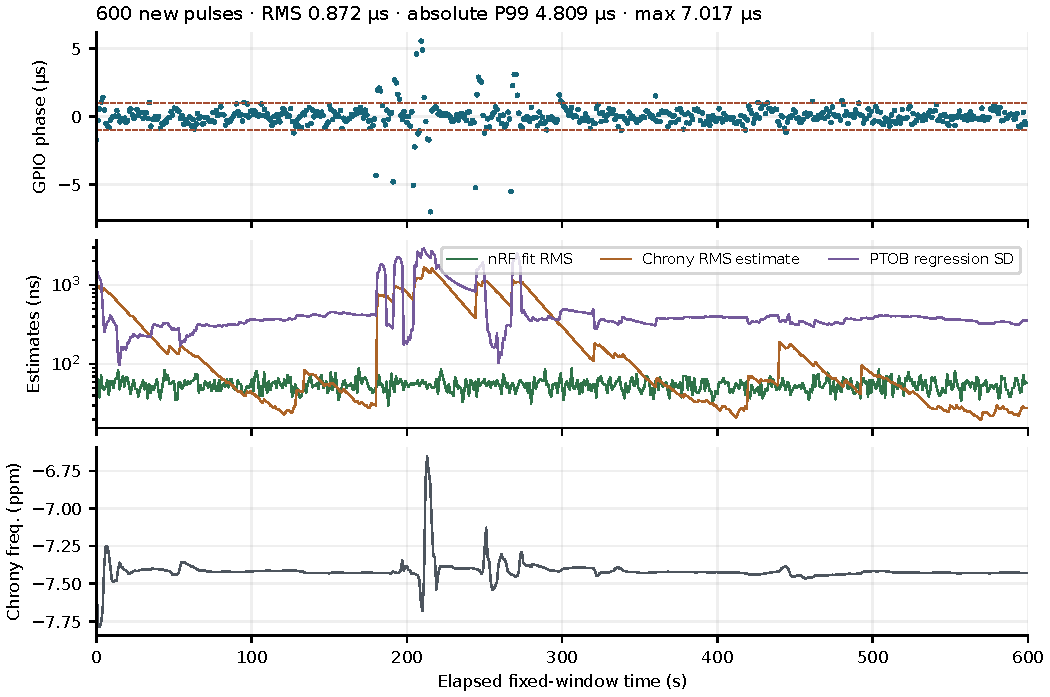
\includegraphics[width=\linewidth]{figures/final-results.pdf}
\caption{The complete final window without error filtering. Dashed lines mark
$\pm1$ \us{} in GPIO phase. The middle panel separates three internal estimates
on a logarithmic scale. The bottom panel shows chrony's frequency estimate;
feedback correlation does not establish the initiating cause of a tail.}
\label{fig:results}
\end{figure}

Across 600 snapshots, the nRF fit RMS had median 54 ns and range 30--88 ns;
chrony's tracking RMS estimate had median 72 ns, mean 256.078 ns and range
20--1670 ns. PTOB regression residual standard deviation had median 371.5 ns
and range 98--2893 ns. There were 597 distinct chrony reference-time updates;
their last-offset RMS was 423.387 ns. Snapshot repetitions are not additional
independent estimates. A small receiver fit residual and a small median chrony
RMS can coexist with microsecond GPIO phase tails, because these quantities
observe different parts of a coupled chain. They cannot identify a GPIO,
radio or servo contribution by subtraction.

\subsection{Network and PHC health boundaries}
The Ethernet cable remained disconnected in all 600 snapshots. A running PHC
transfer and admitted PTP child therefore demonstrate preparation, not Ethernet
delivery. User-space PHC/system midpoint observations had median offset
$+2032.5$ ns, but median read bracket 7102 ns; their uncertain association cannot
qualify sub-microsecond PHC alignment.

A separate bounded post-window check obtained four valid Pi-loopback NTP
responses, all stratum 1 with PTOB reference ID and normal leap status. A
12.006-second passive capture at Pi \code{wlan0} observed 204 PTP egress
packets: 96 matched Sync/Follow\_Up pairs and 12 Announce messages in domain 24.
TAI/realtime read brackets included the operating 37-second offset. These
checks made no clock-setting changes. Loopback NTP and local PTP egress are
protocol-health evidence; no remote receive accuracy or physical Ethernet
performance was measured.

The deidentified full populations, manifest, exact observer source snapshots,
figure script and offline verifier accompany this draft at
\path{evidence/pi5/2026-11-02/} and \path{tools/verify_pi5_gateway.py}.
The verifier recomputes included arithmetic and identities without hardware or
credentials; it cannot re-extract the private raw captures or supply an
independent time reference.

\section{USB as an alternative Pi clock bridge}
The existing macOS client offers a useful architecture, not a drop-in Pi
benchmark \cite{macpaper,macevidence}. On nRF52840, USB SOF events trigger
hardware timer capture. The host resolves the integer frame identity, joins the
hardware frame to its host clock, and evaluates an exact immutable source map.
Retrieval latency does not become the event timestamp. Source boot, counter
epoch, frame identity, map generation and original deadlines fence training.
Current observations are predicted using a preceding fit before entering it.

The historical shared-bus 180-second macOS comparison records corrected-source
RX prediction RMS of 190.050 ns for the BLE RC path, with explicit rejected and
warmup populations. That metric is a causal prediction residual against
SOF/Mach boundaries; it is not absolute UTC or a Pi USB result. The client owns
an unprivileged \code{chronyd -x}; it neither disciplines the macOS system clock
nor serves the network. Its measured transfer chain and API are therefore
different from the current Pi server.

The current M-HAT USB interface supplies diagnostic CDC output; it does not
implement the macOS source contract or a measured Linux SOF bridge.
A Linux port needs more than CDC messages bearing UTC labels. The device must
export captured SOF ordinals/counters and source maps, and the host must prove
which host frame matches which device event. Linux's USB API distinguishes
frame scheduling and URB completion \cite{linuxusb}; a callback arrival or a
frame number alone is not a nanosecond host-clock boundary. A Pi implementation
must characterize its host controller, timestamp association, direct-port/hub
topology, clock crossings, reset/resume and integer-frame ambiguity.
Apple-specific frame/Mach APIs cannot simply be assumed on Linux.

USB could bypass the HAT-to-Pi GPIO IRQ capture and provide a higher observation
rate, while retaining a causal source map. It could also introduce host-controller
latency, frame-association error and shared-bus bias. Millisecond USB frame cadence
does not by itself impose millisecond precision, and hardware SOF on the device
does not by itself guarantee precise host association. An initial Linux prototype
should keep request/completion bounds, unknown bias and invalid samples explicit,
then compare against an independent physical reference before driving system
time. No Pi USB accuracy figure is claimed here.

\section{Reverse direction: external PTP to a PToB mesh}
A reverse gateway would receive time from an external Ethernet PTP domain,
discipline its PHC, bridge that clock to an nRF timer, and publish a new
authenticated PToB source. Hardware-timestamped PTP reception is the first
stage, not the whole transfer. LinuxPTP supports PHC-to-system transfer and
external timestamp synchronization where hardware provides the necessary
pins/channels \cite{phc2sys,ts2phc}. The present server-only configuration must
not be treated as a receiver configuration.

Two candidate bridges are plausible. A suitable NIC/PHC can generate a timed
PPS edge for nRF PPI capture, with separately authenticated second labels and
a measured PHC-to-timer association. This requires an accessible periodic output,
known voltage and edge behavior, counter unwrapping and calibrated delays;
the tested native Pi PHC exposes no such pin. An added obtainable timing NIC or
other hardware would be a separate target requiring measurement. Alternatively,
a causal bidirectional USB/SOF bridge could associate the externally disciplined
host/PHC with the nRF timer. Its uncertainty is presently unknown on this Pi.

The M-HAT receiver firmware cannot currently originate this source. A GM adapter
would need to ingest the bridge, preserve original age and validity, implement
the existing authenticated source/publication contracts, and withdraw when PTP
lock, timescale validity or bridge quality disappears. A UTC second value over
UART is sufficient for labeling only when coupled to a precise, unambiguous
counter event; serial arrival is not that event. The original source's clock
identity and domain must survive translation so that a gateway cannot follow
time that originated from itself through the mesh.

Mode changes require one explicit owner per clock and a drained transition.
In forward mode chrony follows PToB and PHC follows system; in reverse mode
the external PTP receiver owns PHC and a defined process owns system/timer
transfer. Simultaneously following both directions creates a feedback loop.
Fresh source admission, root/boot/epoch changes and TAI--UTC/leap interpretation
must be explicit. The proposal does not configure or operate reverse mode.

\section{Error budgets and practical viability}
A forward conceptual budget contains mesh estimation, radio and board bias,
timer quantization, GPIO capture, system servo and packet transfer:
\[
 e_{\rm out}=e_{\rm mesh}+b_{\rm path}+q_{\rm timer}
              +e_{\rm capture}+e_{\rm servo}+e_{\rm packet}.
\]
The observed \(r_i\) does not identify these terms independently; shared input
and feedback can cancel or amplify them. In particular, subtracting the HAT's
fit RMS in quadrature from GPIO phase RMS would not measure GPIO noise.

For reverse mode, the relevant chain is
\[
 e_{\rm reverse}=e_{\rm PTP\,receive}+e_{\rm PHC\leftrightarrow timer}
                 +e_{\rm publication}+e_{\rm downstream}.
\]
Independent, zero-mean random terms may justify a root-sum-square model after
testing. Unknown or correlated biases need explicit terms, conservative bounds
when justified, and must otherwise remain unknown. Forward phase RMS does not
bound this reverse chain or its tails.

The implemented path is useful as an inspectable mesh-to-Linux integration and
as a way to evaluate time-server applications with stated tolerances.
A continuous error below 1 \us{} is not established by a low median, small
tracking RMS, one stable window or successful NTP/PTP packets. Source changes
and recovery matter to availability; long-run tail rates need more than 600
opportunities. Planned tests are independent PPS/clock comparison, Ethernet
receive/transmit measurements under idle/load and link recovery, longer
same-cohort windows, and matched GPIO versus USB/PHC capture. A reference with
uncertainty below the intended claim and recorded cable/edge delays is necessary.

For a Pi user, the current contribution is a concrete hardware PPS integration,
source-aware diagnostics and conservative NTP/PTP ownership. USB and reverse
PTP ingress are viable architectural research directions whose implementation
and error budgets remain open. Extending the mesh's usability should preserve
those distinctions rather than inheriting precision claims from another host,
transport or internal estimator.

\begin{thebibliography}{12}\small
\bibitem{nordic} Nordic Semiconductor, \emph{nRF52840 Product Specification},
TIMER, PPI, GPIOTE, RADIO and USBD.
\url{https://docs.nordicsemi.com/bundle/ps_nrf52840/page/keyfeatures_html5.html}.
\bibitem{linuxpps} Linux kernel documentation, \emph{PPS support}.
\url{https://docs.kernel.org/driver-api/pps.html}.
\bibitem{ppsgpio} Raspberry Pi Linux, \emph{pps-gpio driver}, rpi-6.18.y.
\url{https://github.com/raspberrypi/linux/blob/rpi-6.18.y/drivers/pps/clients/pps-gpio.c}.
\bibitem{chrony} chrony Project, \emph{chrony.conf(5)}, version 4.6.
\url{https://chrony-project.org/doc/4.6/chrony.conf.html}.
\bibitem{phc2sys} LinuxPTP, \emph{phc2sys(8)}.
\url{https://www.linuxptp.org/documentation/phc2sys/}.
\bibitem{ts2phc} LinuxPTP, \emph{ts2phc(8)}.
\url{https://www.linuxptp.org/documentation/ts2phc/}.
\bibitem{linuxusb} Linux kernel documentation, \emph{The Linux-USB Host Side API}.
\url{https://docs.kernel.org/driver-api/usb/usb.html}.
\bibitem{debiantz} Debian Project, \emph{tzdata README.Debian}, timezone package split.
\url{https://sources.debian.org/src/tzdata/2026c-1/debian/README.Debian}.
\bibitem{macpaper} J. Yantis, \emph{Beyond USB Packet Arrival: Frame-Identified Time Transfer to macOS},
research draft, 17 October 2026, repository canonical source:
\path{papers/usb-macos-time-transfer-preprint.tex}.
\bibitem{macevidence} J. Yantis, \emph{USB timing comparison, 17 October 2026},
selected shared-bus observations and offline verification:
\path{evidence/usb/2026-10-17/README.md}.
\end{thebibliography}
\vspace{0.5em}
{\footnotesize Original paper and figures: CC BY 4.0, Jonathan Yantis.
Draft only; hardware accuracy, reverse mode and Pi USB transfer remain unqualified.}
\end{document}
